\documentclass[12pt]{article}
\usepackage[left=2.5cm, right=1.5cm, top=2cm]{geometry}
\usepackage{amsmath}
\usepackage[document]{ragged2e}
\usepackage[utf8]{inputenc} 
\usepackage[T2A]{fontenc}
\usepackage{color, colortbl}
\usepackage{tabularx}% http://ctan.org/pkg/tabularx
\usepackage{graphicx} % Add pictures to your document
\usepackage[english,ukrainian]{babel} % Українська мова за linux.org.ua
\usepackage{float}
\usepackage{listings}
\usepackage[unicode]{hyperref}
\usepackage{pgfplotstable}
\usepackage{array}
\usepackage{xcolor}
\usepackage{Sweave}
%\usepackage{pgfplots}
%\usepackage{tikz}
\usepackage{makecell}
\usepackage{setspace}
\onehalfspacing
\usepackage[labelsep=period]{caption}
\newcommand{\tabitem}{~~\llap{\textbullet}~~}
\DeclareUnicodeCharacter{0301}{\'{e}}
%\renewcommand\bibname{Список використаних джерел}
\definecolor{bblue}{HTML}{4F81BD}
\definecolor{rred}{HTML}{C0504D}
\definecolor{ggreen}{HTML}{9BBB59}
\definecolor{ppurple}{HTML}{9F4C7C}
\hypersetup{
	colorlinks = true,
	urlcolor = {blue}
}


\definecolor{light-gray}{gray}{0.95}

\lstset{language = c}
\lstset{backgroundcolor = \color{light-gray}}
\lstset{xleftmargin = 1cm}
\lstset{framexleftmargin = 1cm}
\lstset{breaklines=true}
\definecolor{Gray}{rgb}{0.9,0.9,0.9}


\begin{document}
	\section{Introduction}
	\subsection{Purpose}
	Purpose of this document is to describe Chat Service System. This paper will explain the key features of the system, as well as set of interfaces of the system, what the system will do, the constraints under which it must operate and how the system will react to external stimuli, by presenting the general structure and a set of specific use cases. This document is intended for both the stakeholders and the developers of the system.
	\subsection{Scope of project}
	This system is a simple messaging that allows users to register a nickname and post a message that's bundled with such identifier. The system consists of a RESTFul service, a PostgreSQL database and a web-browser Single-Page Application. Database contains messages, users, and active sessions. User's session is defined by a pair of the authentication token and nickname stored in data base, that user is provided as a result of authentication process. User's nickname is bundled to the message through the process of verification of authentication token, that retrieves the respective nickname.
	\subsection{Glossary}
	\begin{table}[H]
		\begin{tabularx}{1.055\textwidth}{|l|l|}
			\firsthline
			Active Article& \makecell{The document that is tracked by the system; it is a narrative \\that is planned to be posted to the public website.} \\
			\hline
			Author & \makecell{Authenticated user with an intent to post \\a prepared message to the board} \\ \hline
			%Author &
			%\makecell{Person submitting an article to be reviewed. \\In case of multiple authors, this term refers to\\ the principal author, with whom all communication is made.} \\ \hline
			Database&
			Collection of all the information monitored by this system.\\ \hline
			%Editor&
			%\makecell{Person who receives articles, sends articles for review, \\and makes final judgments for publications.}\\ \hline
			Field&
			A cell within a form.\\ \hline
			%Historical Society Database&
			%The existing membership database (also HS database).\\ \hline
			Member&
			A member of the Chat service listed in the CSD database.\\ \hline
			Reader&
			Anyone visiting the site to read messages. \\ \hline
			%Review&
			%\makecell{A written recommendation about the appropriateness \\of an article for publication; may include \\suggestions for improvement.} \\ \hline
			%Reviewer&
			%\makecell{A person that examines an article and has \\the ability to recommend approval of the article for \\publication or to request that changes be made in the article.} \\ \hline
			Software Requirements Specification &
			\makecell{A document that completely describes all of the \\functions of a proposed system and the constraints \\under which it must operate. For example, this document.}\\ \hline
			Stakeholder&
			\makecell{Any person with an interest in the project who is \\not a developer.} \\ \hline
			User &
			Author or Reader.\\
			\hline
		\end{tabularx}
	\end{table}
	\section{Overall description}
	\subsection{System enviroment}
	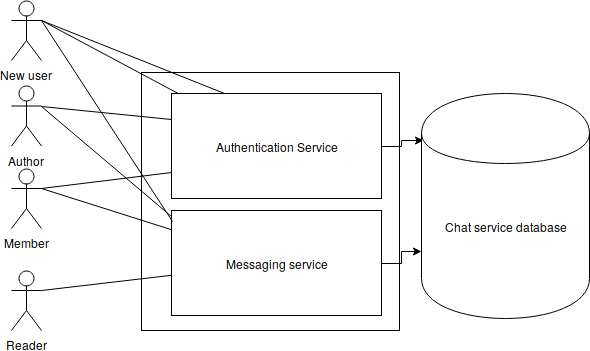
\includegraphics[width=\textwidth]{SystemEnviroment.png}
	RESTFul service consists of two controllers --- Authentication that hands out tokens, and Messaging that puts messages in DB and loads last 50. All users communicate through HTTP requests to specific parts of the server application, for example, /load to load messages
	\subsection{Functional requirement specification}
	This section outlines the use cases for each of the active readers separately. The reader has one use case, the author and the member have three and new user has to go through the process of registration, which is his fourth use case. This paper will present a chart of each user's interaction with requests to REST, and a diagram showcasing the process of each request
	\subsubsection{/load}
	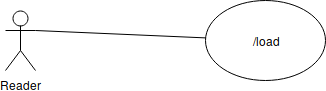
\includegraphics[width=0.5\textwidth]{Reader.png} \\
	Loads messages from database.\\
	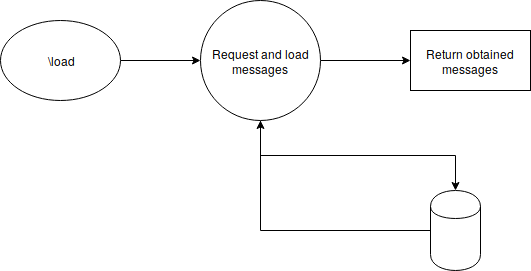
\includegraphics[width=\textwidth]{loadDiagram.png}
	\subsubsection{/register}
	Checks nickname and login availability, then registers user's desired credentials\\
	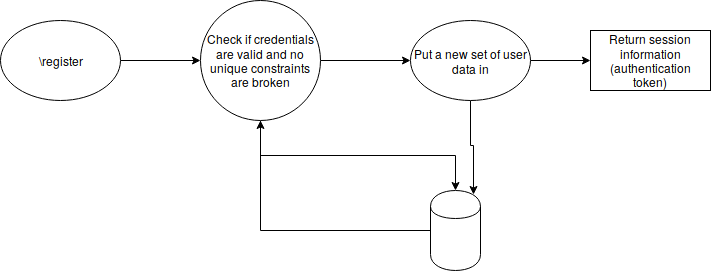
\includegraphics[width=\linewidth]{registerDiagram.png}
	\subsubsection{/auth}
	Authenticates the user and generates authentication token that's associated with user's nickname.\\
	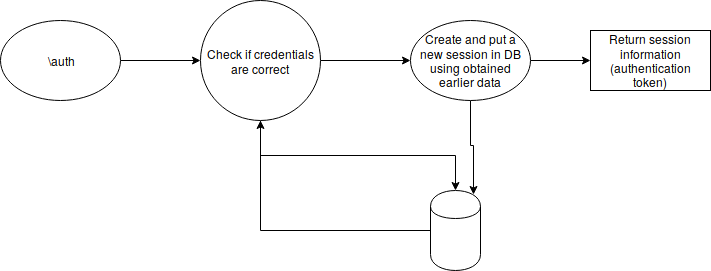
\includegraphics[width=\linewidth]{authDiagram.png}
	\subsubsection{/send}
	Retrieves nickname associated with user's token, and bundles it to the message before posting it to database.\\
	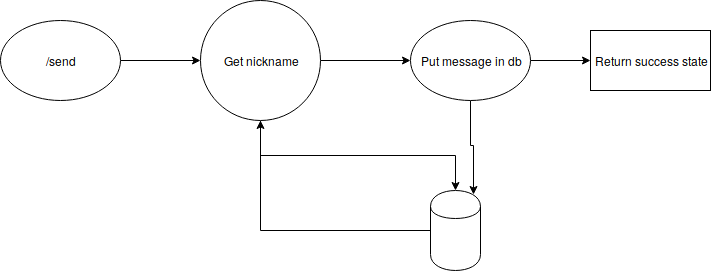
\includegraphics[width=\textwidth]{sendDiagram.png}
	\subsubsection{New user}
	\centering
	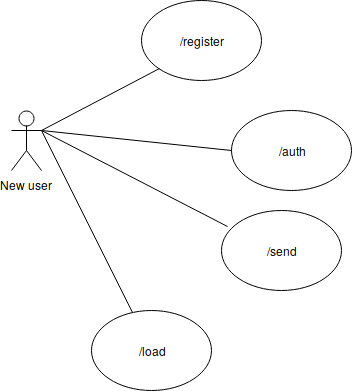
\includegraphics[width=0.5\linewidth]{NewUser.png}
	\flushleft
	\subsubsection{Reader}
	\centering
	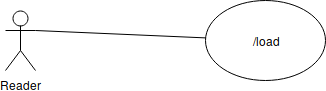
\includegraphics[width=0.5\linewidth]{Reader.png}
	\flushleft
	\subsubsection{Member/Author}
	\centering
	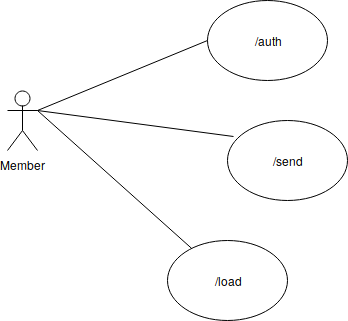
\includegraphics[width=0.5\linewidth]{Member.png}
	\flushleft
	\subsection{Non-Functional requirements}
	The chat service can be installed on a server via on-Premise deployment, given a postgresql database and server are configured beforehand.
\end{document}